\section{Import to Eclipse}
\textit{\hyperref[sec:imp_idea]{Import to IntelliJ Idea}}

\begin{figure}[H]
	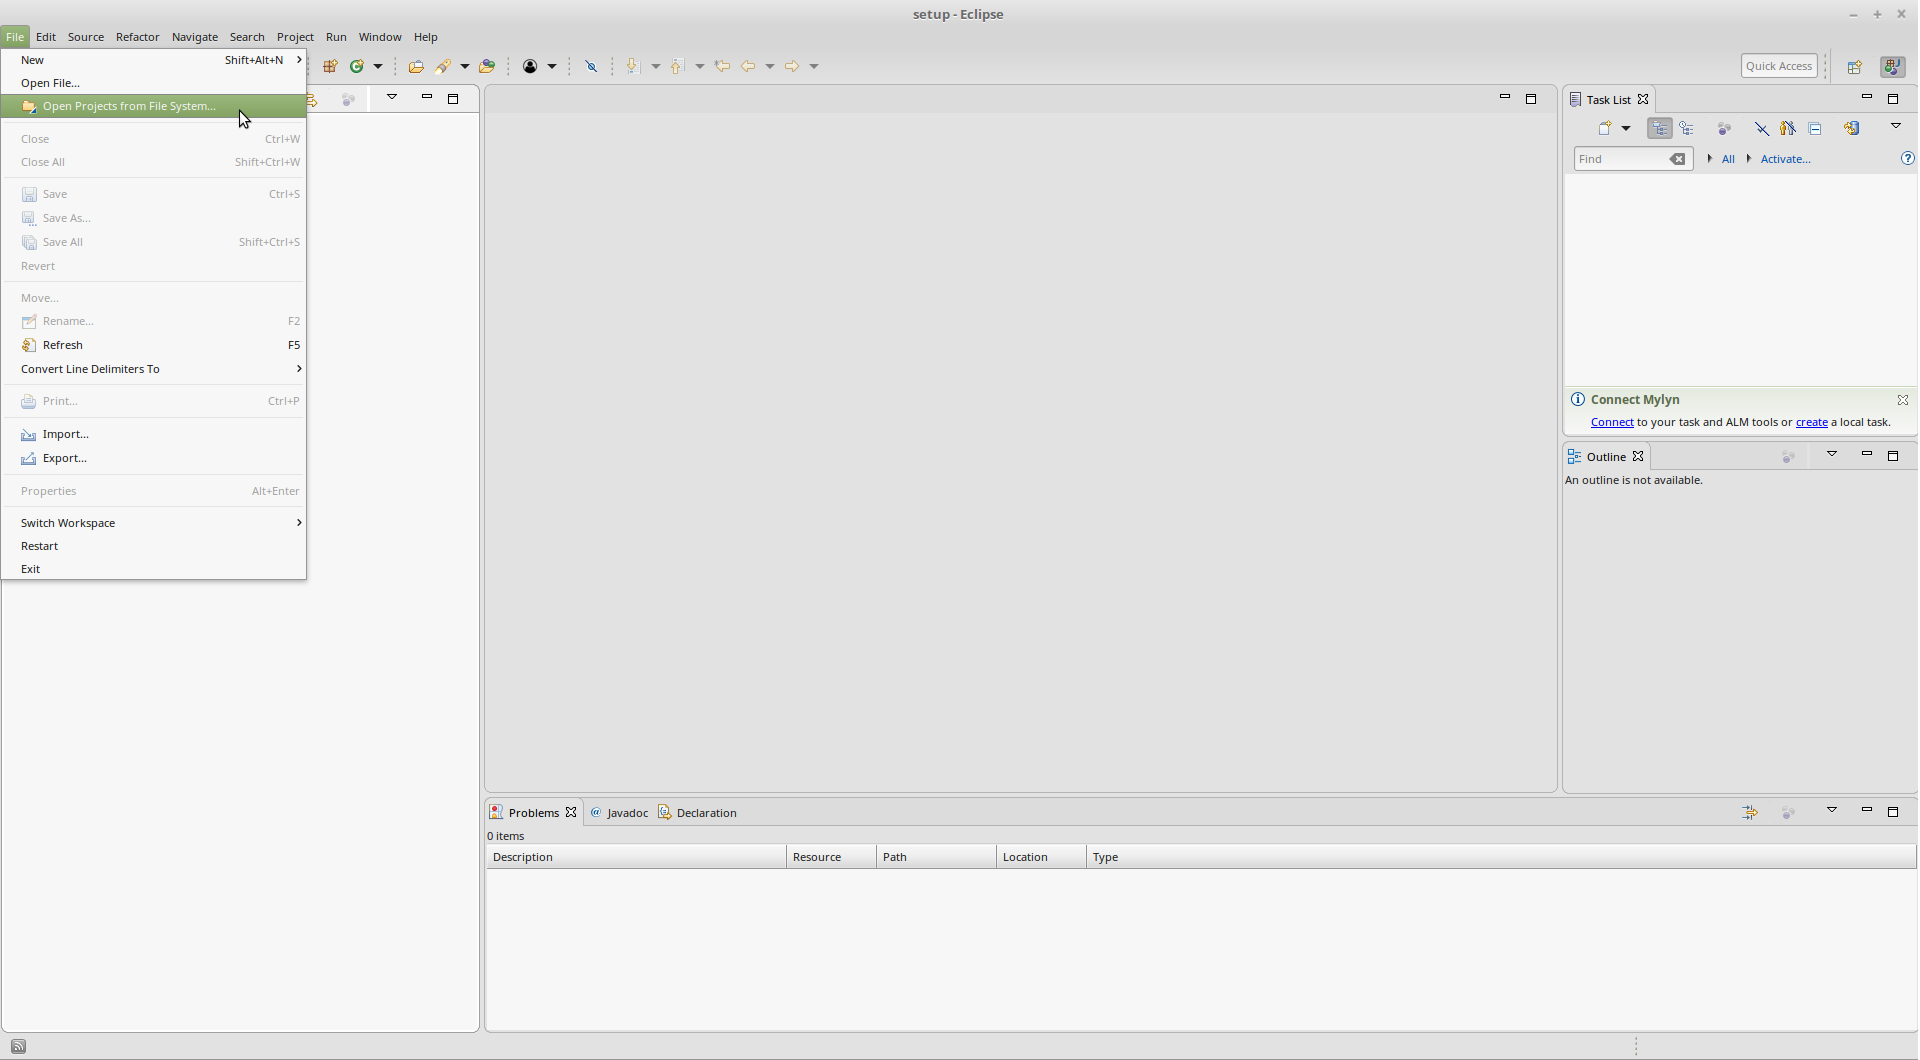
\includegraphics[width=\textwidth]{setup-parts/pictures/eclipse-import-1.png}
	\caption{Click on \textit{"File $\rightarrow$ Open Projects from File System"}}
\end{figure}
\begin{figure}[H]
	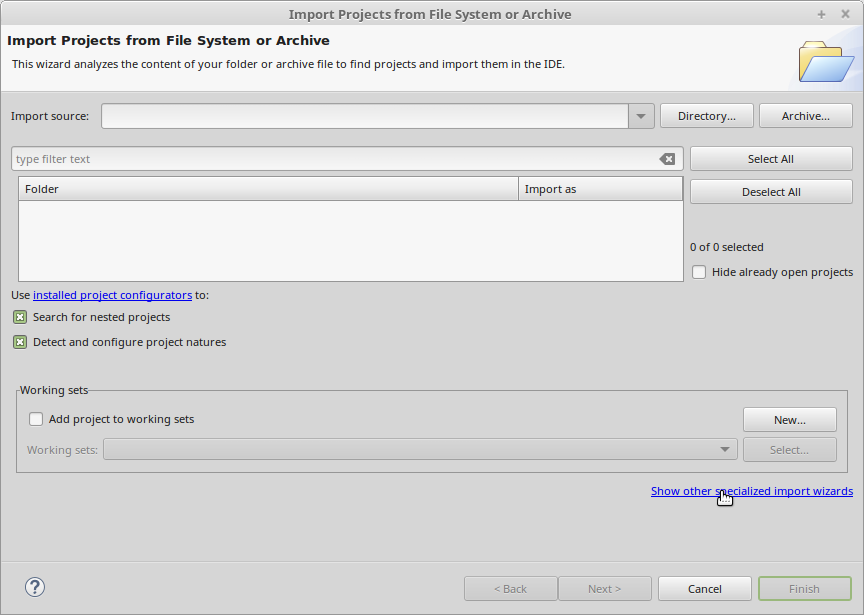
\includegraphics[width=\textwidth]{setup-parts/pictures/eclipse-import-2.png}
	\caption{Click on "\underline{Show other specialized import wizards}"}
\end{figure}
\begin{figure}[H]
	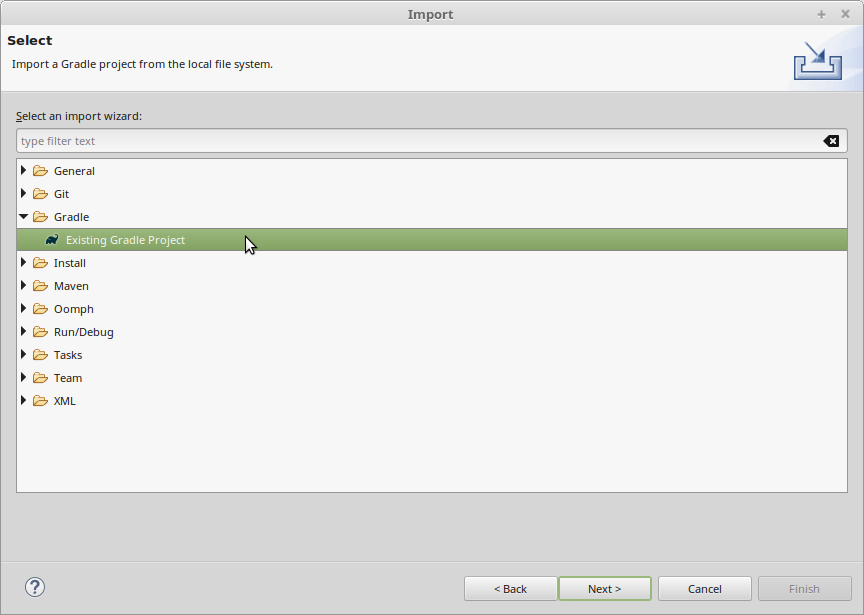
\includegraphics[width=\textwidth]{setup-parts/pictures/eclipse-import-3.png}
	\caption{Select \textit{"Gradle $\rightarrow$ Existing Gradle Project"}}
\end{figure}

\begin{figure}[H]
	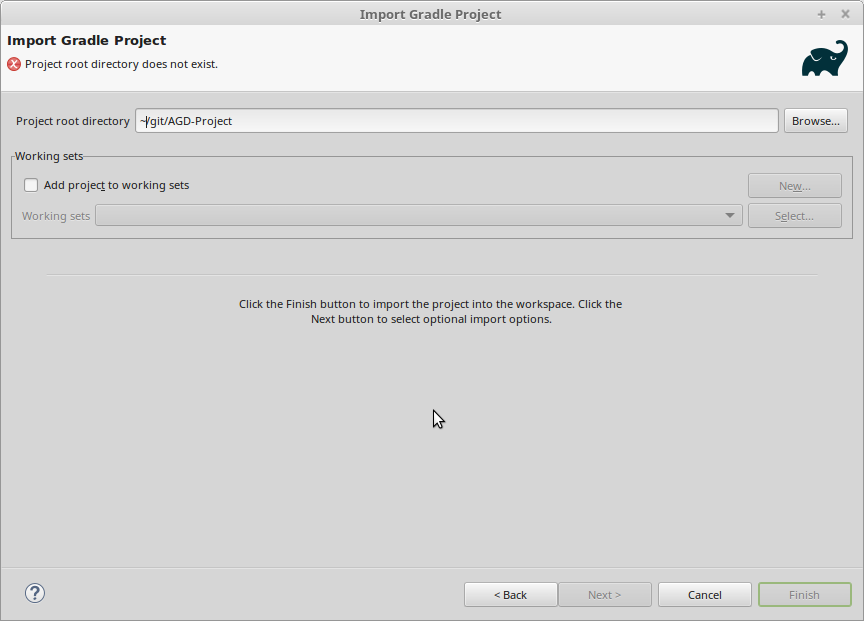
\includegraphics[width=\textwidth]{setup-parts/pictures/eclipse-import-4a.png}
	\caption{Input the folder the Project was cloned into.}
\end{figure}

\begin{figure}
	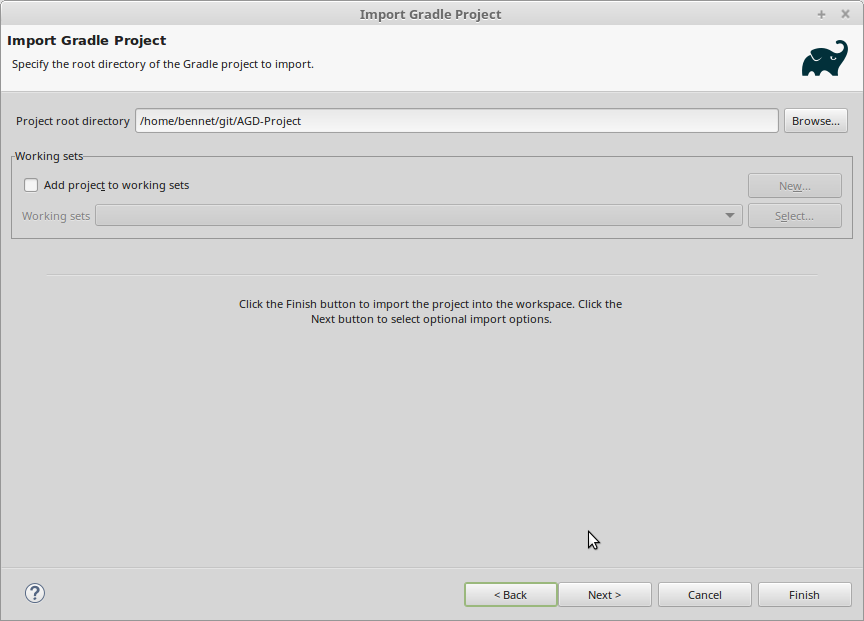
\includegraphics[width=\textwidth]{setup-parts/pictures/eclipse-import-4b.png}
	\caption{You might need to replace a relative path by an absolute one.}
\end{figure}

\begin{figure}[H]
	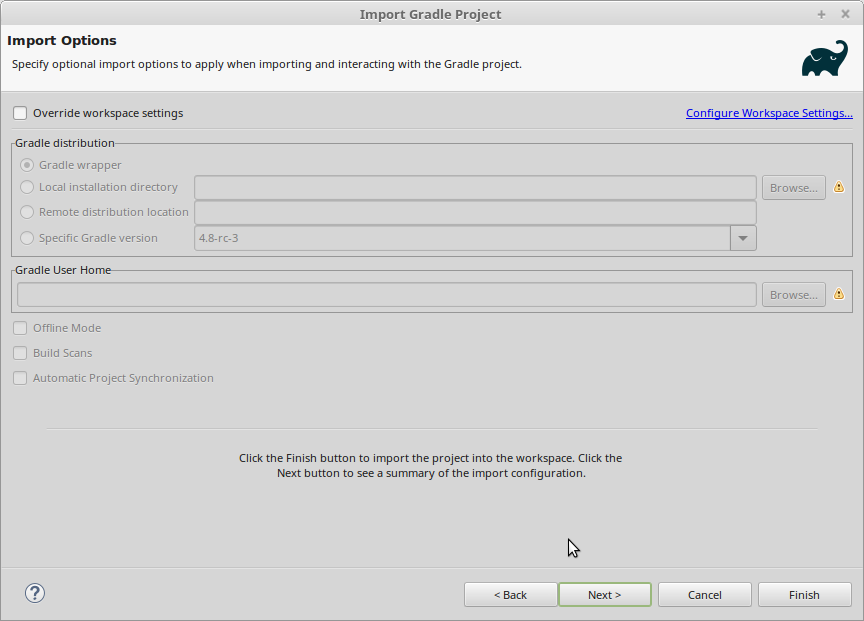
\includegraphics[width=\textwidth]{setup-parts/pictures/eclipse-import-5.png}
	\caption{On the Next Page you can just click "Next"}
\end{figure}
\begin{figure}[H]
	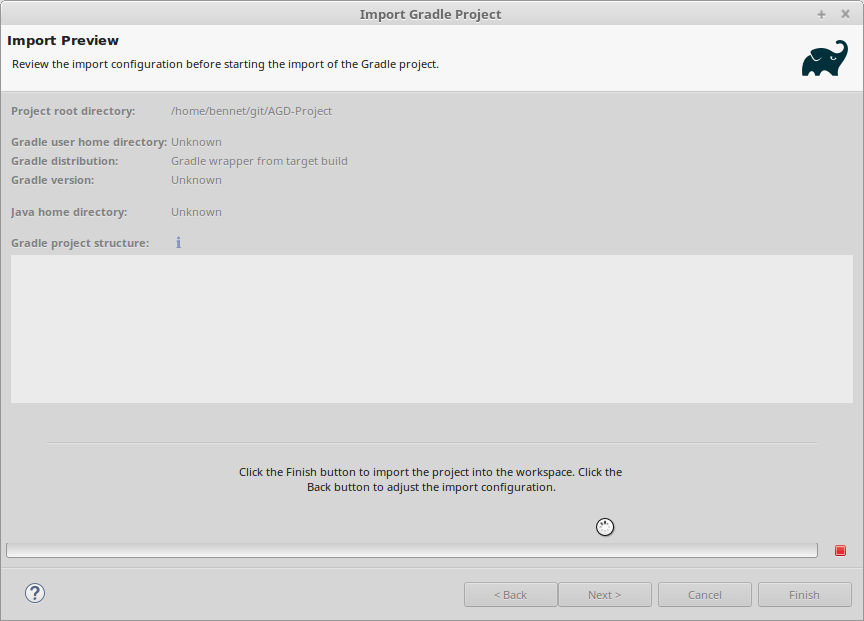
\includegraphics[width=\textwidth]{setup-parts/pictures/eclipse-import-6.png}
	\caption{Wait for gradle to load the Project}
\end{figure}
\begin{figure}[H]
	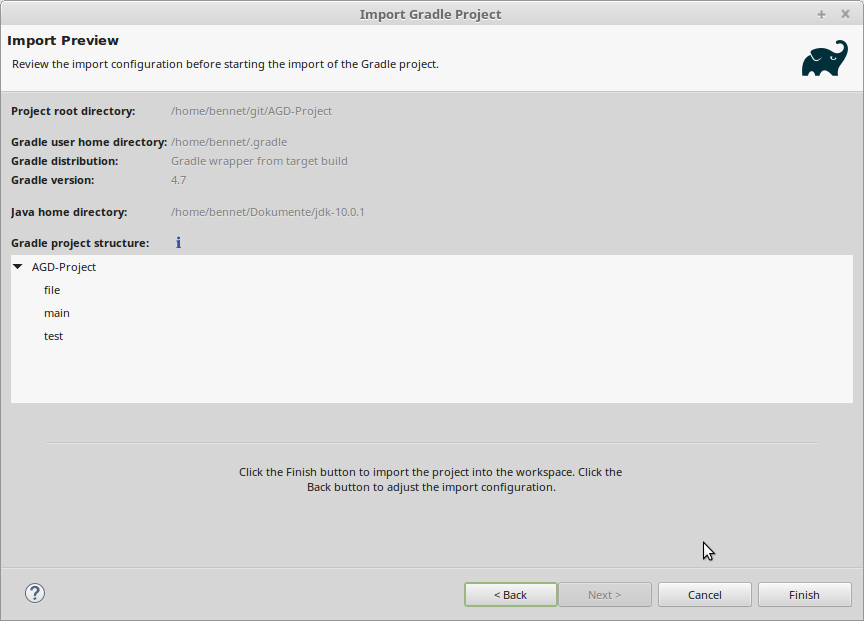
\includegraphics[width=\textwidth]{setup-parts/pictures/eclipse-import-7.png}
	\caption{Click "Finish"}
\end{figure}
\begin{figure}[H]
	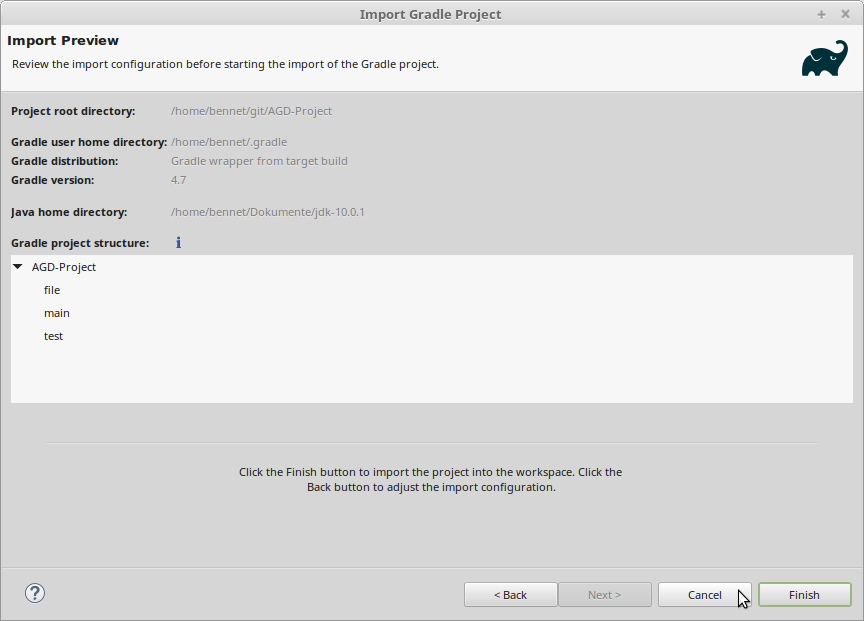
\includegraphics[width=\textwidth]{setup-parts/pictures/eclipse-import-8.png}
	\caption{Click "Cancle" to close the Dialog}
\end{figure}
